

% Options for packages loaded elsewhere
\PassOptionsToPackage{unicode}{hyperref}
\PassOptionsToPackage{hyphens}{url}
%
\documentclass[
  man]{apa6}
\usepackage{lmodern}
\usepackage{amssymb,amsmath}
\usepackage{ifxetex,ifluatex}
\ifnum 0\ifxetex 1\fi\ifluatex 1\fi=0 % if pdftex
  \usepackage[T1]{fontenc}
  \usepackage[utf8]{inputenc}
  \usepackage{textcomp} % provide euro and other symbols
\else % if luatex or xetex
  \usepackage{unicode-math}
  \defaultfontfeatures{Scale=MatchLowercase}
  \defaultfontfeatures[\rmfamily]{Ligatures=TeX,Scale=1}
\fi
% Use upquote if available, for straight quotes in verbatim environments
\IfFileExists{upquote.sty}{\usepackage{upquote}}{}
\IfFileExists{microtype.sty}{% use microtype if available
  \usepackage[]{microtype}
  \UseMicrotypeSet[protrusion]{basicmath} % disable protrusion for tt fonts
}{}
\makeatletter
\@ifundefined{KOMAClassName}{% if non-KOMA class
  \IfFileExists{parskip.sty}{%
    \usepackage{parskip}
  }{% else
    \setlength{\parindent}{0pt}
    \setlength{\parskip}{6pt plus 2pt minus 1pt}}
}{% if KOMA class
  \KOMAoptions{parskip=half}}
\makeatother
\usepackage{xcolor}
\IfFileExists{xurl.sty}{\usepackage{xurl}}{} % add URL line breaks if available
\IfFileExists{bookmark.sty}{\usepackage{bookmark}}{\usepackage{hyperref}}
\hypersetup{
  pdftitle={Theoretical variance, as a function of population parameters},
  pdfauthor={Delacre Marie},
  pdfkeywords={keywords},
  hidelinks,
  pdfcreator={LaTeX via pandoc}}
\urlstyle{same} % disable monospaced font for URLs
\usepackage{graphicx,grffile}
\makeatletter
\def\maxwidth{\ifdim\Gin@nat@width>\linewidth\linewidth\else\Gin@nat@width\fi}
\def\maxheight{\ifdim\Gin@nat@height>\textheight\textheight\else\Gin@nat@height\fi}
\makeatother
% Scale images if necessary, so that they will not overflow the page
% margins by default, and it is still possible to overwrite the defaults
% using explicit options in \includegraphics[width, height, ...]{}
\setkeys{Gin}{width=\maxwidth,height=\maxheight,keepaspectratio}
% Set default figure placement to htbp
\makeatletter
\def\fps@figure{htbp}
\makeatother
\setlength{\emergencystretch}{3em} % prevent overfull lines
\providecommand{\tightlist}{%
  \setlength{\itemsep}{0pt}\setlength{\parskip}{0pt}}
\setcounter{secnumdepth}{-\maxdimen} % remove section numbering
\shorttitle{Theoretical variance}
\affiliation{
\vspace{0.5cm}
\textsuperscript{1} ULB}
\keywords{keywords\newline\indent Word count: X}
\usepackage{csquotes}
\usepackage{upgreek}
\captionsetup{font=singlespacing,justification=justified}

\usepackage{longtable}
\usepackage{lscape}
\usepackage{multirow}
\usepackage{tabularx}
\usepackage[flushleft]{threeparttable}
\usepackage{threeparttablex}

\newenvironment{lltable}{\begin{landscape}\begin{center}\begin{ThreePartTable}}{\end{ThreePartTable}\end{center}\end{landscape}}

\makeatletter
\newcommand\LastLTentrywidth{1em}
\newlength\longtablewidth
\setlength{\longtablewidth}{1in}
\newcommand{\getlongtablewidth}{\begingroup \ifcsname LT@\roman{LT@tables}\endcsname \global\longtablewidth=0pt \renewcommand{\LT@entry}[2]{\global\advance\longtablewidth by ##2\relax\gdef\LastLTentrywidth{##2}}\@nameuse{LT@\roman{LT@tables}} \fi \endgroup}


\DeclareDelayedFloatFlavor{ThreePartTable}{table}
\DeclareDelayedFloatFlavor{lltable}{table}
\DeclareDelayedFloatFlavor*{longtable}{table}
\makeatletter
\renewcommand{\efloat@iwrite}[1]{\immediate\expandafter\protected@write\csname efloat@post#1\endcsname{}}
\makeatother
\usepackage{lineno}

\linenumbers

\title{Theoretical variance, as a function of population parameters}
\author{Delacre Marie\textsuperscript{1}}
\date{}

\begin{document}
\maketitle

\hypertarget{the-variance}{%
\section{The variance}\label{the-variance}}

\hypertarget{cohens-d_s}{%
\subsection{\texorpdfstring{Cohen's \(d_s\)}{Cohen's d\_s}}\label{cohens-d_s}}

\hypertarget{when-variances-are-equal-across-populations}{%
\subsubsection{When variances are equal across populations}\label{when-variances-are-equal-across-populations}}

\hypertarget{when-delta_cohen0}{%
\paragraph{\texorpdfstring{When \(\delta_{Cohen}=0\)}{When \textbackslash delta\_\{Cohen\}=0}}\label{when-delta_cohen0}}

When the population effect size is zero, the variance of Cohen's \(d_s\) can be simplified as follows:

\[Var_{Cohen's \; d_s} = \frac{N(N-2)}{n_1n_2(N-4)}\]

The \textbf{variance} of Cohen's \(d_s\) is a function of total sample size (N) and the sample size allocation ratio (\(\frac{n_1}{n_2}\)):

\begin{figure}
\centering
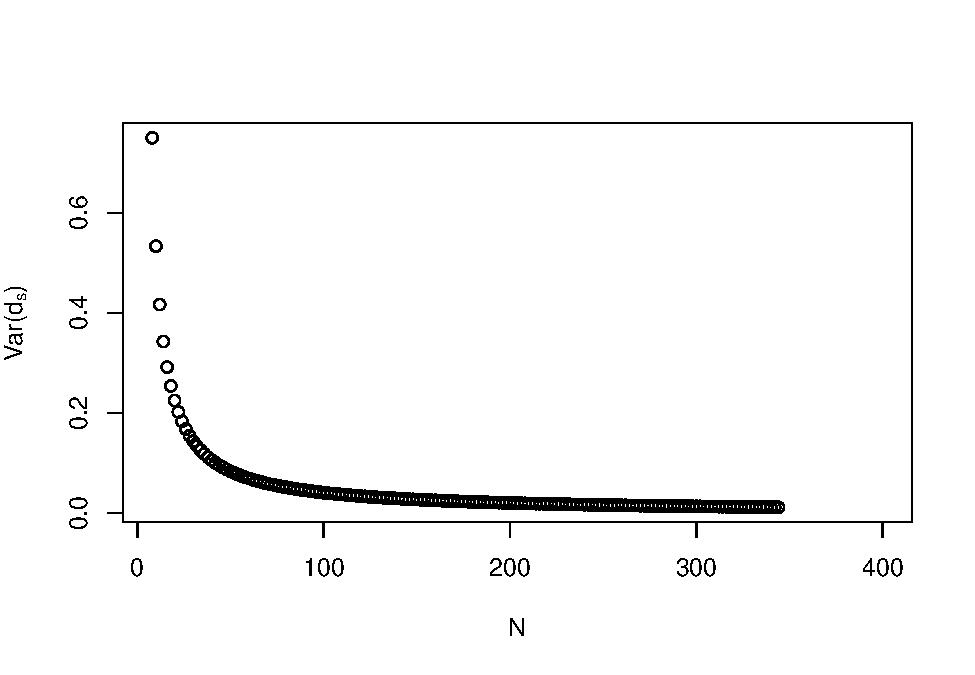
\includegraphics{Theoretical-Variance-of-all-estimators-as-a-function-of-population-parameters_files/figure-latex/varcohendNsize2-1.pdf}
\caption{\label{fig:varcohendNsize2}\ldots{}}
\end{figure}

\begin{itemize}
\tightlist
\item
  The larger the total sample size, the lower the variance. The bias tends to zero when the total sample size tends to infinity (see Figure \ref{fig:varcohendNsize2})
\end{itemize}

\begin{figure}
\centering
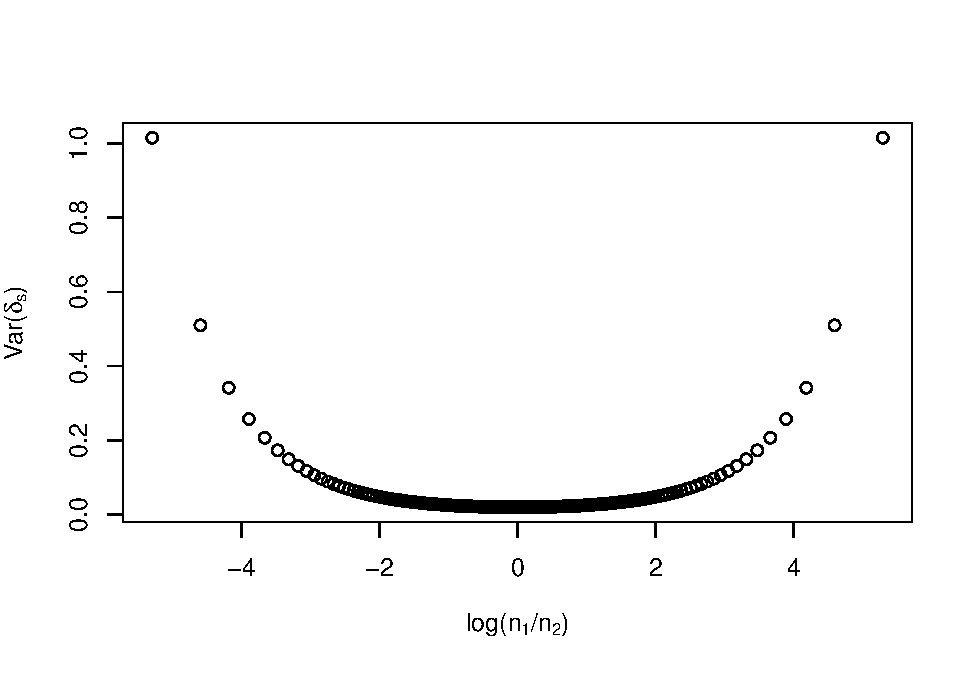
\includegraphics{Theoretical-Variance-of-all-estimators-as-a-function-of-population-parameters_files/figure-latex/varcohenNratio2-1.pdf}
\caption{\label{fig:varcohenNratio2}\ldots{}}
\end{figure}

\begin{itemize}
\tightlist
\item
  The further the sample sizes allocation ratio is from 1, the larger the variance (see Figure \ref{fig:varcohenNratio2})
\end{itemize}

\hypertarget{when-delta_cohen-neq-0}{%
\paragraph{\texorpdfstring{When \(\delta_{Cohen} \neq 0\)}{When \textbackslash delta\_\{Cohen\} \textbackslash neq 0}}\label{when-delta_cohen-neq-0}}

While the variance of \(\delta_{Cohen}\) still depends on the total sample size and the sample sizes allocation ratio, it also depends on the population effect size (\(\delta_{Cohen}\)). The larger the population effect size, the larger the variance. Note that the effect of the population effect size decreases when sample sizes increase, as \(\lim_{n\rightarrow \infty}\left[\frac{df}{df-2} - \left( \frac{\sqrt{\frac{df}{2}} \times \Gamma \left(\frac{df-1}{2} \right)}{\Gamma \left( \frac{df}{2}\right)}\right)^2 \right]=0\).

\hypertarget{glasss-d_s}{%
\subsection{\texorpdfstring{Glass's \(d_s\)}{Glass's d\_s}}\label{glasss-d_s}}

\hypertarget{when-variances-are-equal-across-populations-1}{%
\subsubsection{When variances are equal across populations}\label{when-variances-are-equal-across-populations-1}}

\hypertarget{when-delta_glass0}{%
\paragraph{\texorpdfstring{When \(\delta_{Glass}=0\)}{When \textbackslash delta\_\{Glass\}=0}}\label{when-delta_glass0}}

When the population effect size is zero, the variance of Glass's \(d_s\) can be simplified as follows:

\[Var_{Glass's \; d_s} = \frac{n_c-1}{n_c-3} \left( \frac{1}{n_c}+\frac{1}{n_e}\right)\]

The \textbf{variance} of Glass's \(d_s\) is a function of the sample sizes of both control and experimental group (\(n_c\)) as well as of the sample sizes allocation ratio.

\begin{figure}
\centering
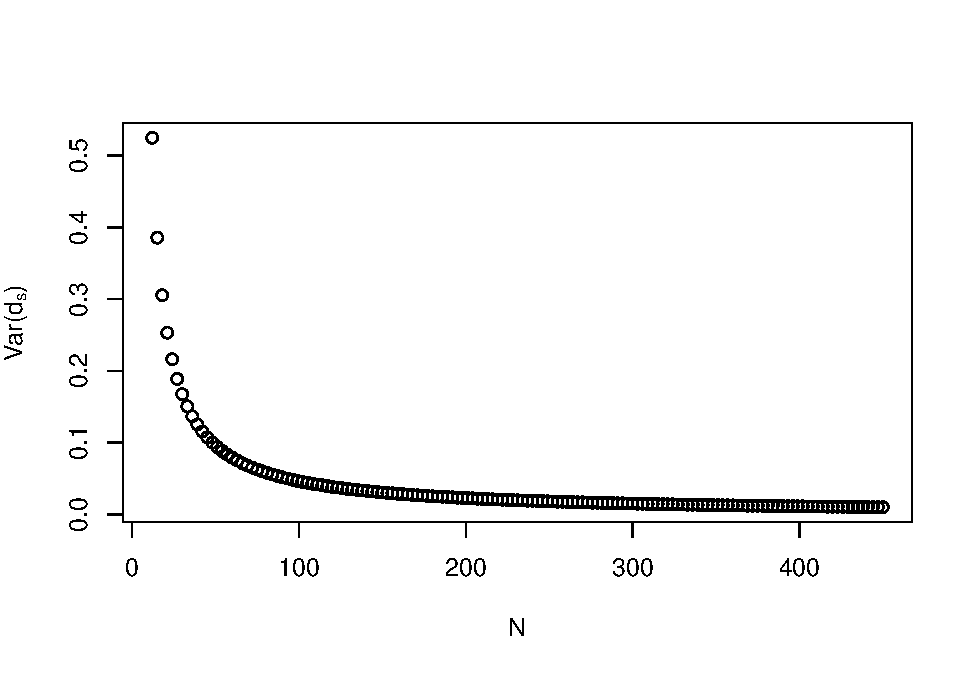
\includegraphics{Theoretical-Variance-of-all-estimators-as-a-function-of-population-parameters_files/figure-latex/varglassNsize2-1.pdf}
\caption{\label{fig:varglassNsize2}\ldots{}}
\end{figure}

\begin{itemize}
\tightlist
\item
  The larger the sample sizes, the lower the variance (Figure \ref{fig:varglassNsize2})
\end{itemize}

\begin{figure}
\centering
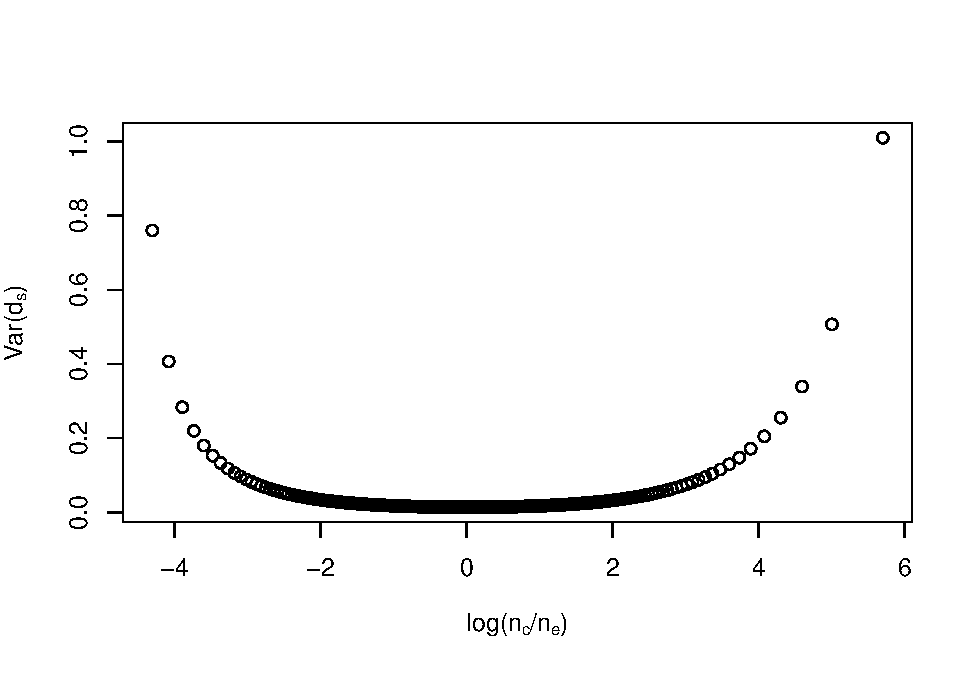
\includegraphics{Theoretical-Variance-of-all-estimators-as-a-function-of-population-parameters_files/figure-latex/varglasshomNratio2-1.pdf}
\caption{\label{fig:varglasshomNratio2}\ldots{}}
\end{figure}

The sample sizes ratio associated with the lowest variance is not exactly 1 (because of the term \(\frac{df}{df-2}\), df depending only on \(n_c\)), but is very close to 1 (and the larger the total sample size, the closer to 1 is the sample sizes ratio associated with the lowest variance).And the further from this sample size ratio, the larger the variance (see Figure \ref{fig:varglasshomNratio2}).

\hypertarget{when-delta_glass-neq-0}{%
\paragraph{\texorpdfstring{When \(\delta_{Glass} \neq 0\)}{When \textbackslash delta\_\{Glass\} \textbackslash neq 0}}\label{when-delta_glass-neq-0}}

\begin{figure}
\centering
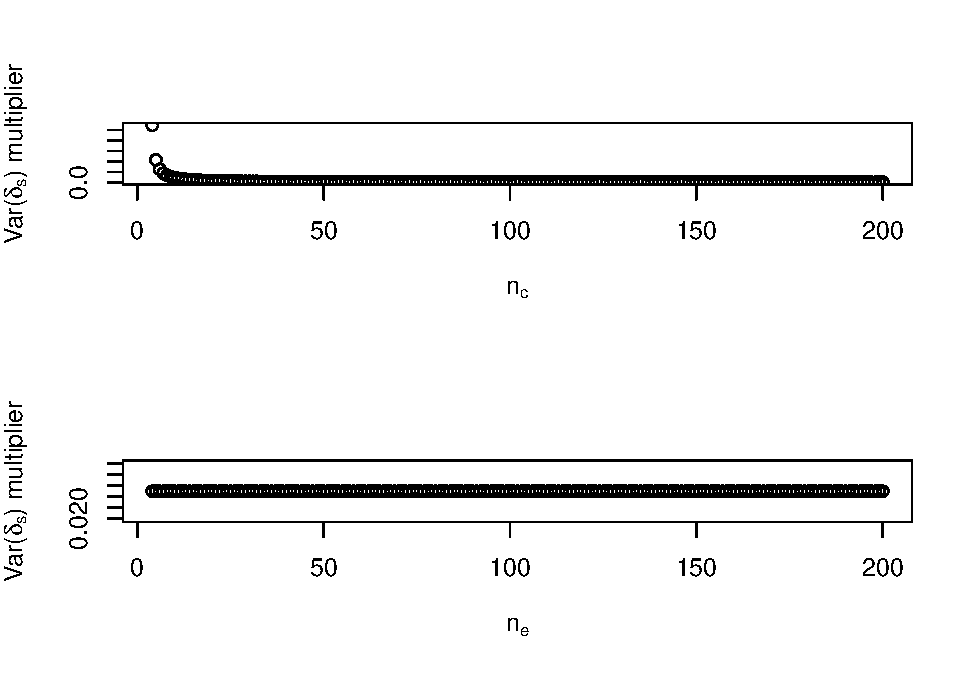
\includegraphics{Theoretical-Variance-of-all-estimators-as-a-function-of-population-parameters_files/figure-latex/varglasswithESNsize2-1.pdf}
\caption{\label{fig:varglasswithESNsize2}\ldots{}}
\end{figure}

While the variance of \(\delta_{Glass}\) still depends on the total sample size and the sample sizes allocation ratio, it also depends on the population effect size (\(\delta_{Cohen}\)). The larger the population effect size, the larger the variance. However, the effect of the population effect size decreases when the control group increases, as \(\lim_{n\rightarrow \infty}\left[\frac{df}{df-2} - \left( \frac{\sqrt{\frac{df}{2}} \times \Gamma \left(\frac{df-1}{2} \right)}{\Gamma \left( \frac{df}{2}\right)}\right)^2 \right]=0\) (see Figure \ref{fig:varglasswithESNsize2}).

\begin{figure}
\centering
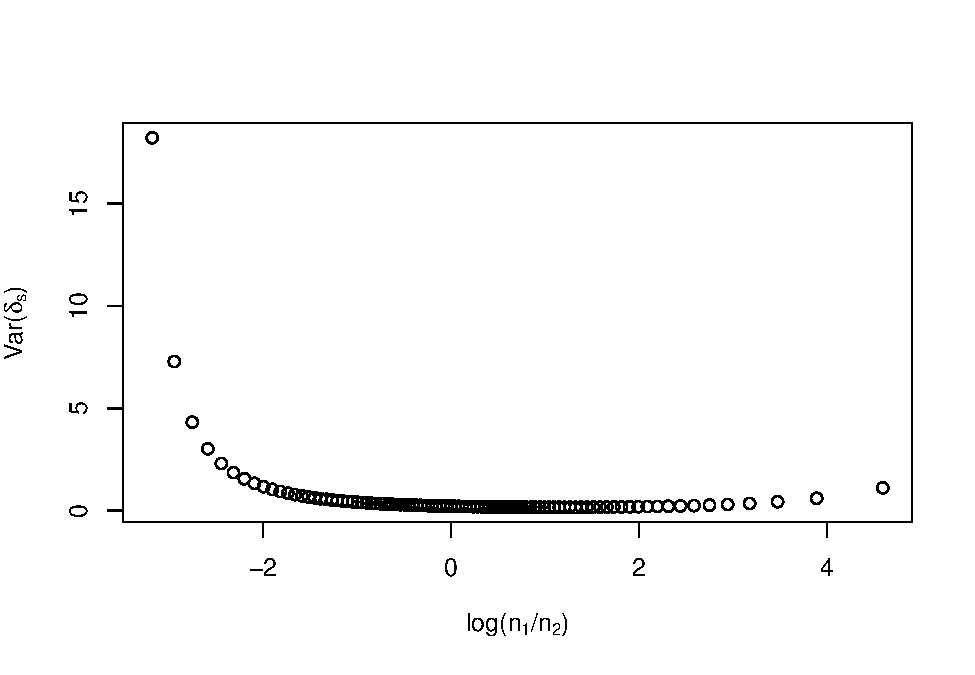
\includegraphics{Theoretical-Variance-of-all-estimators-as-a-function-of-population-parameters_files/figure-latex/varglasshomNratiobis2-1.pdf}
\caption{\label{fig:varglasshomNratiobis2}\ldots{}}
\end{figure}

Note: while the sample sizes ratio associated with the lowest variance was very close to 1 with a null population effect size, this is not true anymore when the population effect size is not zero. Indeed, because of the second term in the adddition, when computing the variance, one gives much more weight to the effect size of the control group (see Figure \ref{fig:varglasshomNratiobis2}), and the larger the population effect size the truer. For example, when \(\delta_{glass}\)= 4, the lowest variance will occure when \(n_c\) is approximately 3 times larger than \(n_e\). When \(\delta_{glass}\)= 7, the lowest variance will occure when \(n_c\) is approximately 5 times larger than \(n_e\), etc.

\hypertarget{when-variances-are-unequal-across-populations-with-equal-sample-sizes}{%
\subsubsection{When variances are unequal across populations, with equal sample sizes}\label{when-variances-are-unequal-across-populations-with-equal-sample-sizes}}

\hypertarget{when-delta_glass0-1}{%
\paragraph{\texorpdfstring{When \(\delta_{Glass}=0\)}{When \textbackslash delta\_\{Glass\}=0}}\label{when-delta_glass0-1}}

When the population effect size is zero, the variance of Glass's \(d_s\) can be simplified as follows:

\[Var_{Glass's \; d_s} = \frac{n-1}{n(n-3)} \left( 1+\frac{\sigma^2_e}{\sigma^2_c}\right)\]

Where \(n=N/2\)=sample size of each group. The variance is therefore a function of the total sample size and the \(SD\)-ratio (\(\frac{\sigma_c}{\sigma_e}\)).

\begin{figure}
\centering
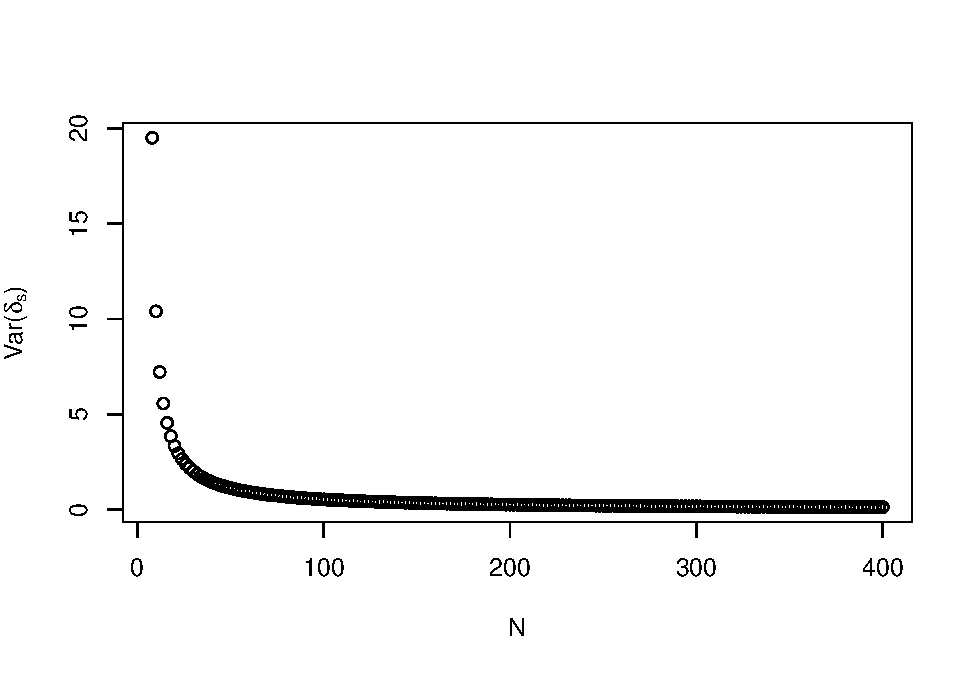
\includegraphics{Theoretical-Variance-of-all-estimators-as-a-function-of-population-parameters_files/figure-latex/varglassHetbalNsize2-1.pdf}
\caption{\label{fig:varglassHetbalNsize2}\ldots{}}
\end{figure}

\begin{itemize}
\tightlist
\item
  The larger the total sample size, the lower the variance (See Figure \ref{fig:varglassHetbalNsize2})
\end{itemize}

\begin{figure}
\centering
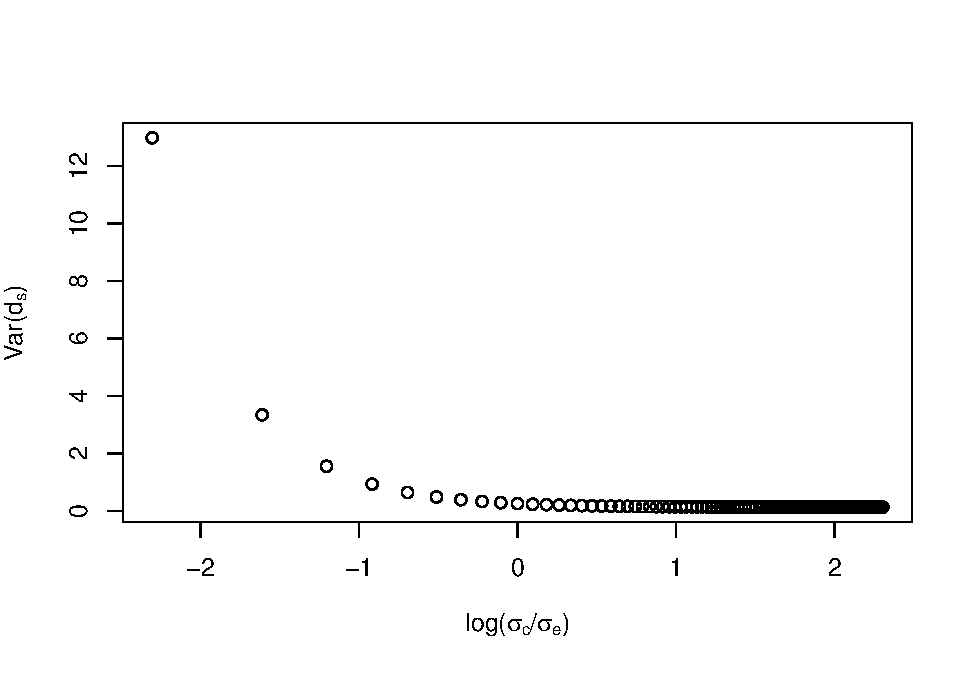
\includegraphics{Theoretical-Variance-of-all-estimators-as-a-function-of-population-parameters_files/figure-latex/varglasshetbalSDratio2-1.pdf}
\caption{\label{fig:varglasshetbalSDratio2}\ldots{}}
\end{figure}

\begin{itemize}
\tightlist
\item
  The larger the \(SD\)-ratio (i.e.~the larger is \(\sigma_c\) in comparison with \(\sigma_e\)), the lower the variance (see Figure \ref{fig:varglasshetbalSDratio2}). However, the effect of the \(SD\)-ratio decreases when sample sizes increase, because \(\lim_{n\rightarrow \infty}\left[\frac{n-1}{n(n-3)} \right]=0\).
\end{itemize}

\hypertarget{when-delta_glass-neq-0-1}{%
\paragraph{\texorpdfstring{When \(\delta_{Glass} \neq 0\)}{When \textbackslash delta\_\{Glass\} \textbackslash neq 0}}\label{when-delta_glass-neq-0-1}}

While the variance of \(\delta_{Glass}\) still depends on the total sample size and the \(SD\)-ratio, it also depends on the population effect size (\(\delta_{Glass}\)). The larger the population effect size, the larger the variance. However, the effect of the population effect size decreases when the control group increases, as \(\lim_{n\rightarrow \infty}\left[\frac{df}{df-2} - \left( \frac{\sqrt{\frac{df}{2}} \times \Gamma \left(\frac{df-1}{2} \right)}{\Gamma \left( \frac{df}{2}\right)}\right)^2 \right]=0\) (see Figure \ref{fig:varglasswithESNsize2}).

\hypertarget{when-variances-are-unequal-across-populations-with-unequal-sample-sizes}{%
\subsubsection{When variances are unequal across populations, with unequal sample sizes}\label{when-variances-are-unequal-across-populations-with-unequal-sample-sizes}}

\hypertarget{when-delta_glass0-2}{%
\paragraph{\texorpdfstring{When \(\delta_{Glass}=0\)}{When \textbackslash delta\_\{Glass\}=0}}\label{when-delta_glass0-2}}

When the population effect size is zero, the variance of Glass's \(d_s\) can be simplified as follows:

\[Var_{Glass's \; d_s} = \frac{n_c-1}{n_c-3} \left( \frac{1}{n_c}+\frac{\sigma^2_e}{n_e\sigma^2_c}\right)\]

The variance of Glass's \(d_s\) is therefore a function of the total sample size (N), the \(SD\)-ratio and the interaction between the sample sizes ratio and the \(SD\)-ratio.

\begin{figure}
\centering
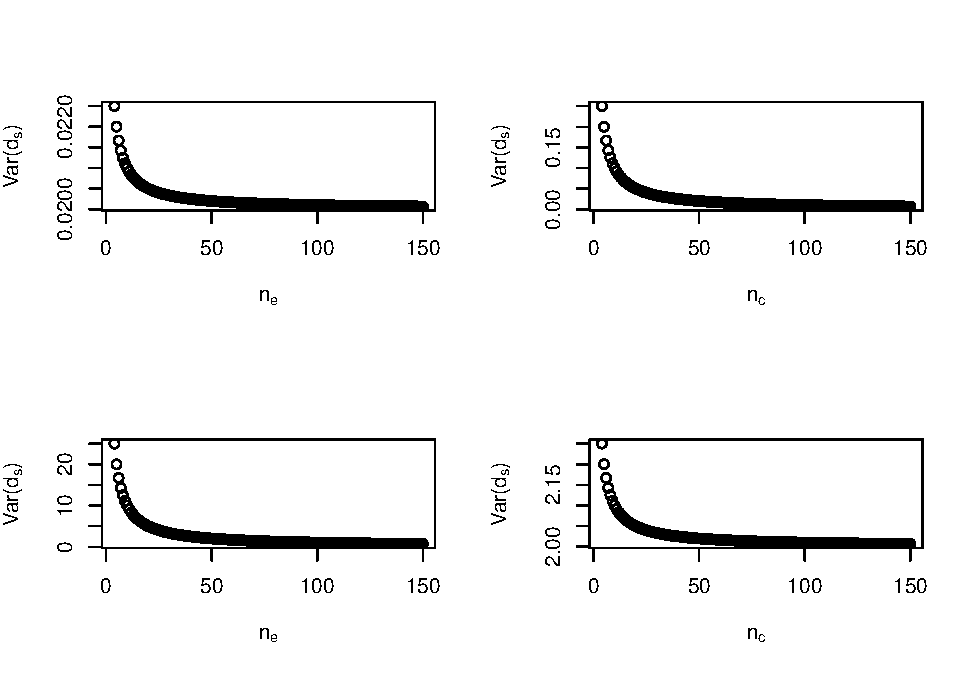
\includegraphics{Theoretical-Variance-of-all-estimators-as-a-function-of-population-parameters_files/figure-latex/varglassHetunbalNsize2-1.pdf}
\caption{\label{fig:varglassHetunbalNsize2}\ldots{}}
\end{figure}

\begin{itemize}
\tightlist
\item
  Whatever the \(SD\) and sample sizes pairing, increasing \(n_c\) and/or \(n_e\) will decrease the variance (see Figure \ref{fig:varglassHetunbalNsize2}).
\end{itemize}

\begin{figure}
\centering
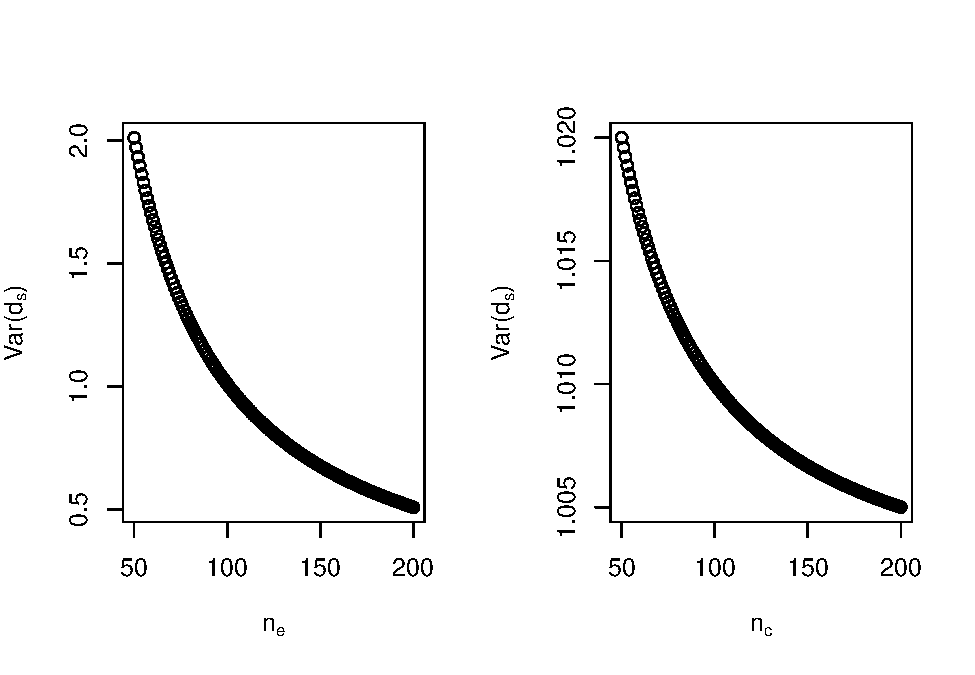
\includegraphics{Theoretical-Variance-of-all-estimators-as-a-function-of-population-parameters_files/figure-latex/varglassHetunbalNwhensdelargerthansdc2-1.pdf}
\caption{\label{fig:varglassHetunbalNwhensdelargerthansdc2}\ldots{}}
\end{figure}

\begin{figure}
\centering
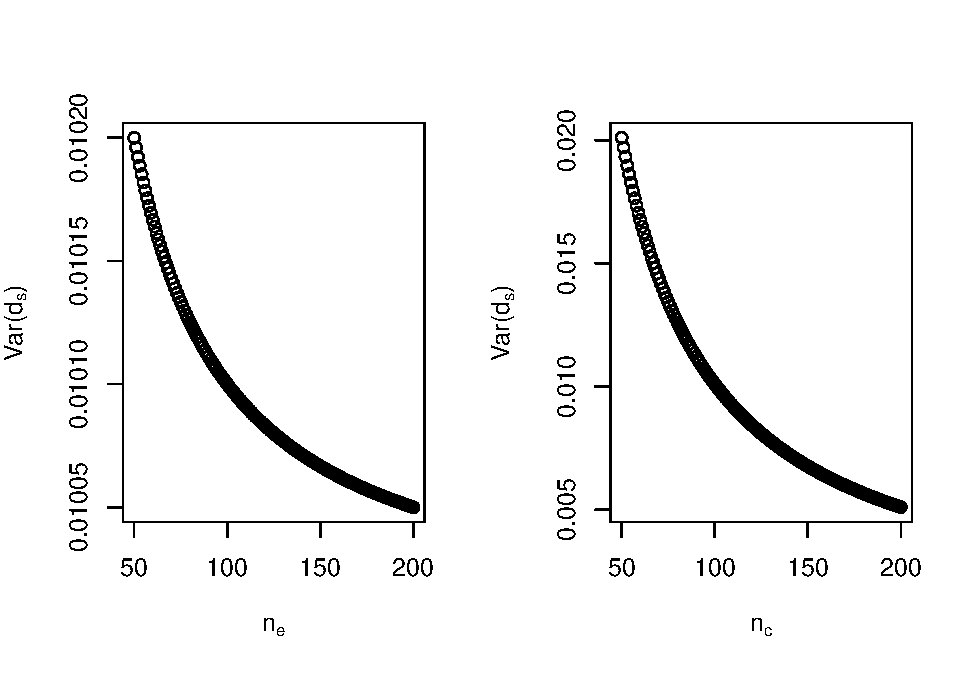
\includegraphics{Theoretical-Variance-of-all-estimators-as-a-function-of-population-parameters_files/figure-latex/varglassHetunbalNwhensdclargerthansde2-1.pdf}
\caption{\label{fig:varglassHetunbalNwhensdclargerthansde2}\ldots{}}
\end{figure}

\begin{itemize}
\tightlist
\item
  The effect of the sample sizes ratio depends on the \(SD\)-ratio:

  \begin{itemize}
  \tightlist
  \item
    We previously mentioned that when \(\sigma_c=\sigma_e\), the variance is minimized when sample sizes of both groups are almost identical (see Figure \ref{fig:varglasshomNratio2}), meaning that it is more efficient, in order to reduce variance, to add subjects uniformly in both groups;\\
  \item
    When \(\sigma_e > \sigma_c\), more weight is given to \(n_e\), meaning that it is more efficient, in order to reduce variance, to add subjects in the experiental group (\(n_e\); see Figure \ref{fig:varglassHetunbalNwhensdelargerthansdc2});\\
  \item
    When \(\sigma_c > \sigma_e\), less weight is given to \(n_e\), meaning that it is more efficient, in order to reduce variance, to add sujects in the control group (\(n_c\); see Figure \ref{fig:varglassHetunbalNwhensdclargerthansde2}).
  \end{itemize}
\end{itemize}

\begin{figure}
\centering
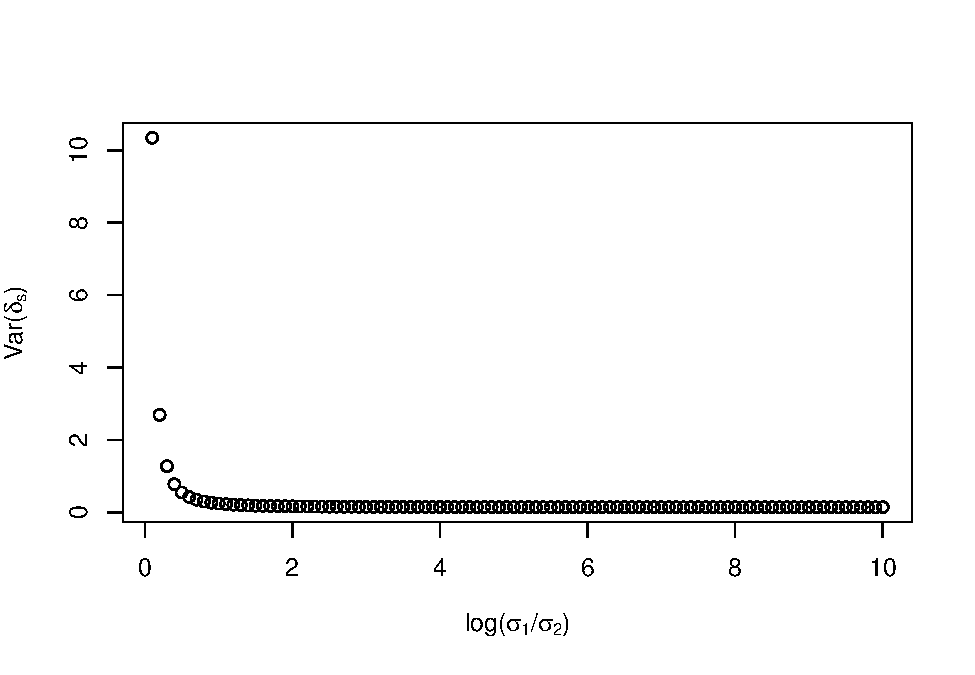
\includegraphics{Theoretical-Variance-of-all-estimators-as-a-function-of-population-parameters_files/figure-latex/varglasshetunbalSDratio2-1.pdf}
\caption{\label{fig:varglasshetunbalSDratio2}\ldots{}}
\end{figure}

\begin{itemize}
\tightlist
\item
  Finally, there is also a main effect of the \(SD\)-ratio: the larger is \(\sigma_c\) in comparison with \(\sigma_e\), the lower the variance, as we can observe in Figure \ref{fig:varglasshetunbalSDratio2}
\end{itemize}

Note that the effect of the \(SD\)-ratio, and the interaction effect between \(SD\)-ratio and sample sizes ratio decreases when the sample size of the control group increases (because \(\frac{n_c-1}{n_c-3}\) get closer to 1).

\hypertarget{when-delta_glass-neq-0-2}{%
\paragraph{\texorpdfstring{When \(\delta_{Glass} \neq 0\)}{When \textbackslash delta\_\{Glass\} \textbackslash neq 0}}\label{when-delta_glass-neq-0-2}}

While the variance of \(\delta_{Glass}\) still depends on the total sample size, the \(SD\)-ratio and the interaction between the \(SD\)-ratio and the sample sizes ratio, it also depends on the population effect size (\(\delta_{Glass}\)): the larger the population effect size, the larger the variance. However, the effect of the population effect size decreases when the sample size of the control group increases, as \(\lim_{n\rightarrow \infty}\left[\frac{df}{df-2} - \left( \frac{\sqrt{\frac{df}{2}} \times \Gamma \left(\frac{df-1}{2} \right)}{\Gamma \left( \frac{df}{2}\right)}\right)^2 \right]=0\)

Note: when the population effect size was null, when \(\sigma_e>\sigma_c\), it was much more efficient to add subjects in the experimental group in order to reduce the variance (because much more weight were given to \(n_e\)). When \(\delta_{Glass} \neq 0\), it is important to add subjects in both groups in order to reduce the variance (because \(\frac{df}{df-2} - \left( \frac{\sqrt{\frac{df}{2}} \times \Gamma \left(\frac{df-1}{2} \right)}{\Gamma \left( \frac{df}{2}\right)}\right)^2\) is only a function of the sample size of the control group). With huge population effect size, it is even always more important to add subjects in the control group (e.g.~when \(\delta_{Glass}=30\)).

\end{document}
